\documentclass{article}
%% Chapter 2 Section 4: Adjoints

\usepackage{amsmath}
\usepackage{amssymb}
\usepackage{hyperref}
\usepackage{mathpartir}
\usepackage{palatino}
\usepackage{tikz}


\newcommand{\one}{\mathbf{1}}
\newcommand{\ccat}{\mathbf{C}}
\newcommand{\dcat}{\mathbf{D}}
\newcommand{\id}{\mathbf{id}}
\newcommand{\pifun}{\mathbf{\Pi}}
\newcommand{\diagfun}{\mathbf{\Delta}}

\newcommand{\eval}{\emph{eval}}
\newcommand{\curry}{\emph{\curry}}

\newcommand{\ints}{\mathbb{Z}}
\newcommand{\reals}{\mathbb{R}}
\newcommand{\ceil}[1]{\lceil #1 \rceil}
\newcommand{\floor}[1]{\lfloor #1 \rfloor}

\begin{document}

\begin{enumerate}
\item [2.4.5]
  \begin{description}
  \item [Unit:]
    The unit diagram operates on the distinguished object $*$ of the category $\one$ and arbitrary objects $y$ of the category $\ccat$.
    Like Pierce said, the functor $F : \one \rightarrow \ccat$ is the left adjoint of the constant functor $T : \ccat \rightarrow \one$.
    Additionally the unit $\iota : \id_\one \rightarrow \id_\one$ is fixed.
    \begin{center}
      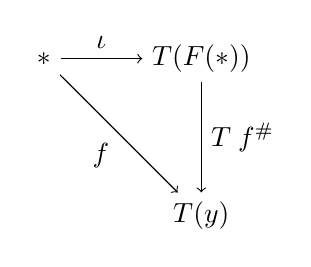
\begin{tikzpicture}
        \node (1) {$*$};
        \node [right of=1, xshift=1cm] (2) {$T(F(*))$};
        \node [below of=2, yshift=-1cm] (3) {$T(y)$};
        
        \draw[->] (1) -- node [above] {$\iota$} (2);
        \draw[->] (1) -- node[below left] {$f$} (3);
        \draw[->] (2) -- node [right] {$T~f^{\#}$} (3);
      \end{tikzpicture}
    \end{center}
    For each object of $\one$, each object of $\ccat$, and each $\one$-arrow $f: X \rightarrow T(y)$ there is a unique $\ccat$ arrow $f^{\#} : F(*) \rightarrow y$.
    Because there is only one object in the category $\one$, we have that for each object in $\ccat$ there is a unique arrow $f^{\#}$ taking the image of $*$ to this object $y$.
    Thus the image of $*$ must be an initial object.

    Existence and uniqueness follow from the existence and uniqueness of $f = \id_*$ in the category $\one$.

  \vfill{}
  \item [Co-unit:]
    Similarly, the counit diagram works in the opposite direction.
    \begin{center}
      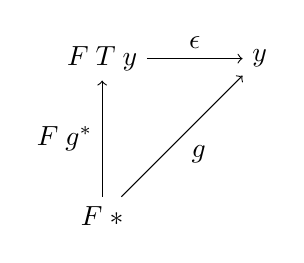
\begin{tikzpicture}
        \node (1) {$F~T~y$};
        \node [below of=1, yshift=-1cm] (2) {$F~*$};
        \node [right of=1, xshift=1cm] (3) {$y$};
        \draw[->] (2) -- node [left] {$F~g^*$} (1);
        \draw[->] (1) -- node[above] {$\epsilon$} (3);
        \draw[->] (2) -- node [below right] {$g$} (3);
      \end{tikzpicture}
    \end{center}
    We have that for each $y \in \ccat$ the counit $\epsilon$ picks out the unique arrow from the initial object $F~*$ to $y$.
    Existence and uniqueness follow because $F*$ is an initial object in $\ccat$.
  \end{description}
  \vfill{}
\newpage
\item[2.4.7]
  We have a category $\ccat$ with products, a product functor $\pifun : \ccat \times \ccat \rightarrow \ccat$ and a diagonal functor $\diagfun :\ccat \rightarrow \ccat \times \ccat$.
  The diagram for the unit is:
  \begin{center}
    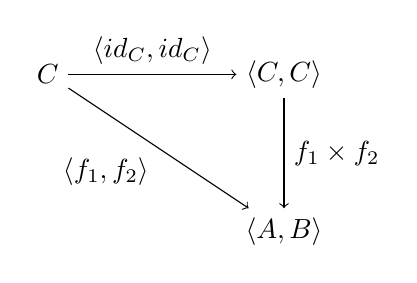
\begin{tikzpicture}
      \node (1) {$C$};
      \node[right of=1,xshift=2cm] (2) {$\langle C , C \rangle$};
      \node[below of=2,yshift=-1cm] (3) {$\langle A , B \rangle$};

      \draw[->] (1) -- node[above] {$\langle id_C, id_C \rangle$} (2);
      \draw[->] (1) -- node[below left] {$\langle f_1 , f_2 \rangle$} (3);
      \draw[->] (2) -- node[right] {$f_1 \times f_2$} (3);
    \end{tikzpicture}
  \end{center}
  The important thing to remember is that $C$, $\langle C , C \rangle$, and $\langle A , B \rangle$ are all objects in $\ccat$.
  The difference between the $\ccat$-arrow $\langle f_1 , f_2 \rangle$ and the $\ccat \times \ccat$-arrow $f_1 \times f_2$ is that the latter is the image of the former under the product functor $\pifun$.
  Existence and uniqueness follow by the existence and uniqueness of the arrow $\langle f_1, f_2 \rangle$.

  The diagram for the counit is conversely between objects of $\ccat \times \ccat$.
  We represent these with parenthesis rather than angle braces, so $(C,C) \in \ccat \times \ccat$ and $\langle C , C \rangle \in \ccat$.
  \begin{center}
    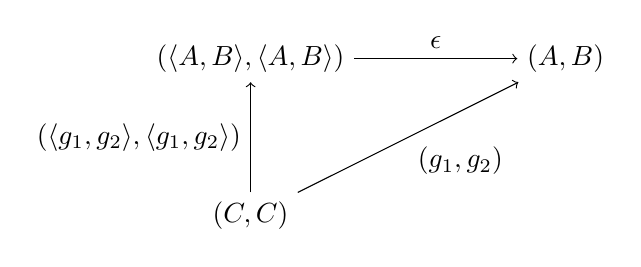
\begin{tikzpicture}
      \node (1) {$(\langle A , B \rangle , \langle A , B \rangle)$};
      \node [below of=1,yshift=-1cm] (2) {$(C, C)$};
      \node [right of=1,xshift=3cm] (3) {$(A, B)$};
      
      \draw[->] (2) -- node[left] {$(\langle g_1 , g_2 \rangle , \langle g_1 , g_2 \rangle)$} (1);
      \draw[->] (2) -- node[below right] {$(g_1, g_2)$} (3);
      \draw[->] (1) -- node[above] {$\epsilon$} (3);
    \end{tikzpicture}
  \end{center}
  The counit $\epsilon$ must be the pair of projections $(\pi_1 , \pi_2) \in \ccat \times \ccat$.
  The existence and uniqueness of the arrow $(\langle g_1 , g_2 \rangle , \langle g_1 , g_2 \rangle)$ follows from the universal mapping property of the product $A \times B$.
  If $C$ is such that we have arrows $g_1 : C \rightarrow A$ and $g_2 : C \rightarrow B$:

  \begin{center}
    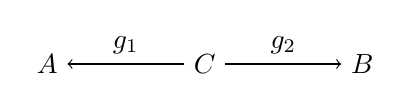
\begin{tikzpicture}
      \node (1) {$C$};
      %% \node [below of=1,yshift=-1cm] (2) {$ $};
      \node [left of=1,xshift=-1cm] (3) {$A$};
      \node [right of=1,xshift=1cm] (4) {$B$};

      \draw[->] (1) -- node[above] {$g_1$} (3);
      \draw[->] (1) -- node[above] {$g_2$} (4);
    \end{tikzpicture}
  \end{center}

  Then there exists a unique mediating arrow $\langle g_1 , g_2 \rangle$ such that the following diagram commutes.
  \begin{center}
    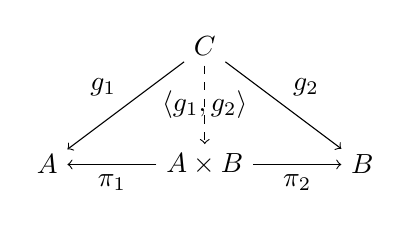
\begin{tikzpicture}
      \node (1) {$C$};
      \node [below of=1,yshift=-0.5cm] (2) {$A \times B$};
      \node [left of=2,xshift=-1cm] (3) {$A$};
      \node [right of=2,xshift=1cm] (4) {$B$};

      \draw[->] (1) -- node[above left] {$g_1$} (3);
      \draw[->] (1) -- node[above right] {$g_2$} (4);
      \draw[->] (2) -- node[below] {$\pi_1$} (3);
      \draw[->] (2) -- node[below] {$\pi_2$} (4);
      \draw[->,dashed] (1) -- node {$\langle g_1,g_2 \rangle$} (2);
    \end{tikzpicture}
  \end{center}


\newpage
\item[2.4.12.1] %% dualize the initial objects to get terminal objects
  Exercise \textbf{2.4.5} showed how an initial object in a category $\ccat$ arises as the image of the unique object $*$ of the category $\one$ under a left adjoint to the constant functor $T : \ccat \rightarrow \one$.
  
  Dually, a final object 1 in a category $\ccat$ arises as the \emph{preimage} of the unique object $*$ of the category $\one$ under a \emph{right} adjoint to the constant functor $T$.
  The unit picks out the unique $\ccat$-arrow from any $\ccat$-object to the final object, 1, and the counit is fixed as $I_\one \rightarrow I_\one$.
  
  The unit and counit diagrams are below.
  The functor $G : \one \rightarrow \ccat$ maps the object $*$ to the final object $1$ in $\ccat$.
  \begin{center}
      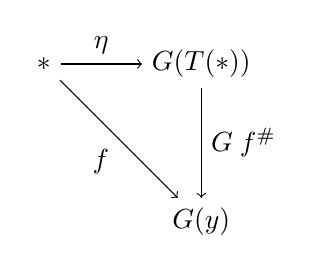
\begin{tikzpicture}
        \node (1) {$*$};
        \node [right of=1, xshift=1cm] (2) {$G(T(*))$};
        \node [below of=2, yshift=-1cm] (3) {$G(y)$};
        
        \draw[->] (1) -- node [above] {$\eta$} (2);
        \draw[->] (1) -- node[below left] {$f$} (3);
        \draw[->] (2) -- node [right] {$G~f^{\#}$} (3);
      \end{tikzpicture}
      \hspace{2cm}
      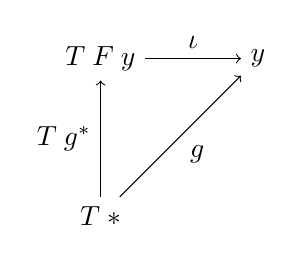
\begin{tikzpicture}
        \node (1) {$T~F~y$};
        \node [below of=1, yshift=-1cm] (2) {$T~*$};
        \node [right of=1, xshift=1cm] (3) {$y$};
        \draw[->] (2) -- node [left] {$T~g^*$} (1);
        \draw[->] (1) -- node[above] {$\iota$} (3);
        \draw[->] (2) -- node [below right] {$g$} (3);
      \end{tikzpicture}
  \end{center}

  The existence and uniqueness of the arrow $f^{\#}$ follows because $1$ is a final object in $\ccat$.
  Hence there exists a unique arrow for each $C \in \ccat$ mapping $C$ to $1$.

\subitem  
  The existence and uniqueness of the arrow $g^*$ follows by the existence and uniqueness of the identity arrow $\id_*$ in the category $\one$.

\vfill{}
\item[2.4.12.2]
  The categorical coproduct is the left adjoint to the diagonal functor $\diagfun$.
  The unit of the adjunction carries a $\ccat$-object to its product and the counit of the adjuction collapses the identity coproduct into a $\ccat$-object.
  \begin{center}
      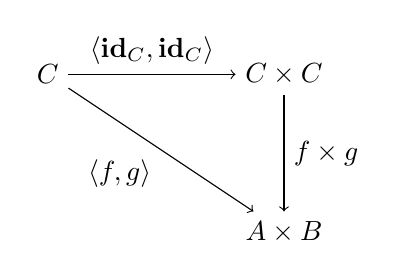
\begin{tikzpicture}
        \node (1) {$C$};
        \node [right of=1, xshift=2cm] (2) {$C \times C$};
        \node [below of=2, yshift=-1cm] (3) {$A \times B$};
        
        \draw[->] (1) -- node [above] {$\langle \id_C , \id_C \rangle$} (2);
        \draw[->] (1) -- node[below left] {$\langle f, g \rangle$} (3);
        \draw[->] (2) -- node [right] {$f \times g$} (3);
      \end{tikzpicture}
      \hspace{1cm}
      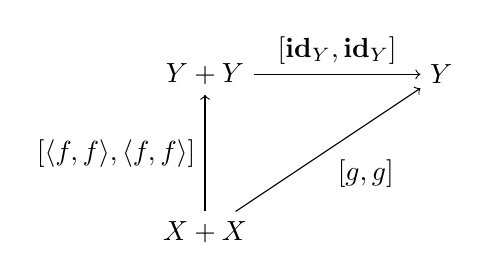
\begin{tikzpicture}
        \node (1) {$Y + Y$};
        \node [below of=1, yshift=-1cm] (2) {$X + X$};
        \node [right of=1, xshift=2cm] (3) {$Y$};
        \draw[->] (2) -- node [left] {$[\langle f, f \rangle, \langle f, f \rangle]$} (1);
        \draw[->] (1) -- node[above] {$[\id_Y , \id_Y]$} (3);
        \draw[->] (2) -- node [below right] {$[g,g]$} (3);
      \end{tikzpicture}
  \end{center}

\vfill{}
\newpage
\item[2.4.12.3]
  Example \textbf{2.4.8} showed that $\eval_{AB}$ was the counit of the adjunction between the functors $F = (- \times A)$ and $G = (-)^A$.
  The counit diagram Pierce gave was the diagram for an exponential object $B^A$.
  %% \begin{center}
  %%     \begin{tikzpicture}
  %%       \node (1) {$B^A \times A$};
  %%       \node [below of=1, yshift=-1cm] (2) {$C \times A$};
  %%       \node [right of=1, xshift=2cm] (3) {$B$};
  %%       \draw[->] (2) -- node [left] {$g$} (1);
  %%       \draw[->] (1) -- node[above] {$\eval_{AB}$} (3);
  %%       \draw[->] (2) -- node [below right] {$\curry(g) \times \id_A$} (3);
  %%     \end{tikzpicture}
  %% \end{center}

\subitem
  The unit of this adjunction is the class of arrows that take a fixed $\ccat$-object $C$ to the pair of a $\ccat$-object $A$ and $\ccat$-arrows from $A$ to $C$.
  The mapping from $f$ to $f^{\#}$ is the process of uncurrying a function $f : C \rightarrow A \rightarrow B$ into a function $f^{\#} : C \times A \rightarrow B$.
  \begin{center}
      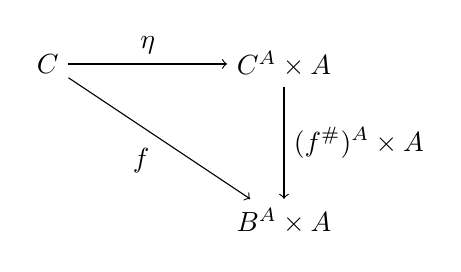
\begin{tikzpicture}
        \node (1) {$C$};
        \node [right of=1, xshift=2cm] (2) {$C^A \times A$};
        \node [below of=2, yshift=-1cm] (3) {$B^A \times A$};
        
        \draw[->] (1) -- node [above] {$\eta$} (2);
        \draw[->] (1) -- node[below left] {$f$} (3);
        \draw[->] (2) -- node [right] {$(f^{\#})^A \times A$} (3);
      \end{tikzpicture}
  \end{center}

\vfill{}
\item[2.4.12.4]
  Just as the ceiling functor $\ceil{} : \ints \rightarrow \reals$ is the left adjoint of the inclusion functor $U : \ints \rightarrow \reals$, we can show that the floor functor $\floor{} : \reals \rightarrow \ints$ is the right adjoint to the inclusion $U$.
  The unit of the adjunction represents the fact that for all integers $N$, the inequality $N \le \floor{U(N)}$ holds.
  \begin{center}
    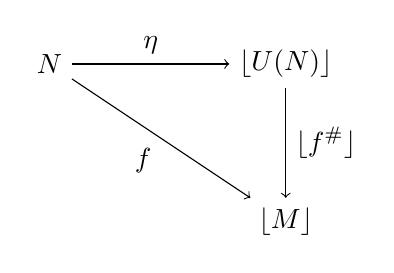
\begin{tikzpicture}
      \node (1) {$N$};
      \node [right of=1, xshift=2cm] (2) {$\floor{U(N)}$};
      \node [below of=2, yshift=-1cm] (3) {$\floor{M}$};
      
      \draw[->] (1) -- node [above] {$\eta$} (2);
      \draw[->] (1) -- node[below left] {$f$} (3);
      \draw[->] (2) -- node [right] {$\floor{f^{\#}}$} (3);
    \end{tikzpicture}
  \end{center}
  Here, the function $f$ is any map between integers.
  The unique $f^*$ arises from the definition of the floor function: namely that the floor of a real number $r$ is the \emph{greatest} integer less than $r$.

\vfill{}
\newpage
\item[2.4.12.5]
  We first show how the unit and counit of an adjunction uniquely determine one another.
%% , we consider an adjoint pair of $(F,G)$ as an isomorphism of hom-sets.
%%   $$\dcat(F(X),Y) \approx \ccat(X,G(Y))$$
%%   Schematically, this is equivalent to:
%%   \begin{mathpar}
%%     \inferrule{
%%       F(X) \rightarrow Y
%%     }{
%%       X \rightarrow G(Y)
%%     }
%%   \end{mathpar}

\subitem
  Assume first the we have $\eta : X \rightarrow G(F(X))$, the unit of the adjunction, and want to derive the counit $\epsilon$.
  Diagramatically, the unit gives the following picture.
  \begin{center}
      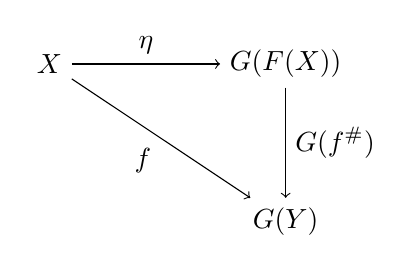
\begin{tikzpicture}
        \node (1) {$X$};
        \node [right of=1, xshift=2cm] (2) {$G(F(X))$};
        \node [below of=2, yshift=-1cm] (3) {$G(Y)$};
        
        \draw[->] (1) -- node [above] {$\eta$} (2);
        \draw[->] (1) -- node[below left] {$f$} (3);
        \draw[->] (2) -- node [right] {$G(f^{\#})$} (3);
      \end{tikzpicture}
  \end{center}
\subitem
  The object $X$ stands for any arbitrary object in the domain of $G$ (or equally, the codomain of $F$).
  Fix $X$ to be $G(Y)$.
  This yields a new picture where $f$ is the identity $\id_{G(Y)}$.
  \begin{center}
      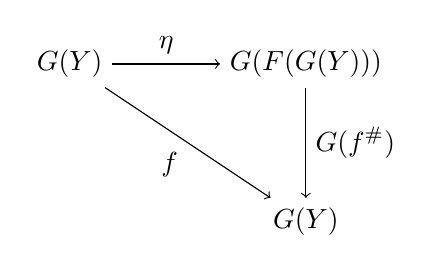
\begin{tikzpicture}
        \node (1) {$G(Y)$};
        \node [right of=1, xshift=2cm] (2) {$G(F(G(Y)))$};
        \node [below of=2, yshift=-1cm] (3) {$G(Y)$};
        
        \draw[->] (1) -- node [above] {$\eta$} (2);
        \draw[->] (1) -- node[below left] {$f$} (3);
        \draw[->] (2) -- node [right] {$G(f^{\#})$} (3);
      \end{tikzpicture}
  \end{center}
\subitem
  The unit $\eta$ uniquely determines an arrow $f^{\#} : F(G(Y)) \rightarrow Y$.
  This is the counit of the adjunction. %% TODO needs proving

\subitem
  Conversely, if we assume we have the counit $\epsilon : F(G(Y)) \rightarrow Y$ then by fixing $Y = F(X)$ we uniquely determine $g*$ as the unit of the adjunction.
  In the corresponding diagram, $g$ is the identity on $F(X)$ and $g^*$ is uniquely determined by the counit.

\subitem
  If we look at the adjoint structure as a natural transformation between hom-functors, Pierce explains that we can represent the adjoint schematically as:
  \begin{mathpar}
    \inferrule{
      F(X) \rightarrow Y
    }{
      X \rightarrow G(Y)
    }
  \end{mathpar}
  Filling in $Y = F(X)$ on the left and $X = G(Y)$ on the right, it's easier to see how the unit and counit are determined.
  \begin{mathpar}
    \inferrule{
      F(X) \rightarrow F(X)
    }{
      X \rightarrow G(F(X))
    }
  \end{mathpar}
  \begin{mathpar}
    \inferrule{
      F(G(Y)) \rightarrow Y
    }{
      G(Y) \rightarrow G(Y)
    }
  \end{mathpar}
\subitem
  The arrow from $X$ to $G(F(X))$ is the unit and the arrow from $F(G(Y))$ to $Y$ is the counit.
  Thanks to \href{http://www.andrew.cmu.edu/user/awodey/}{Professor Awodey's} \href{http://www.youtube.com/watch?v=r0YOAeDJ9tU&index=10&list=PLGCr8P_YncjVjwAxrifKgcQYtbZ3zuPlb}{lectures} from \href{https://www.cs.uoregon.edu/research/summerschool/summer14/}{OPLSS} for showing this.

\subitem
  Because the unit and counit uniquely determine one another, it follows that the functors $F$ and $G$ determine one another to within a natural isomorphism.
  If we know $F$ is the left adjoint of some other functor, there is only one choice (up to isomorphism) of $G$ that will satisfy the necessary requirements.
  Likewise if we know $G$ and derive $F$.

\end{enumerate}
\end{document}
